\chapter{ARTE COMPUTACIONAL E INTERATIVIDADE}

\section{DA CONTEMPLAÇÃO À INTERAÇÃO}

De acordo com \citeonline[p. 97]{frechiani}, historicamente, dentre as tendências que situam a importância do espectador na costituição da obra, a arte percorreu um caminho até finalmente desembocar no universo da interatividade. Esse percurso parte da contemplação, onde o fruidor é um agente passivo, passa pela participação ativa, onde encontramos a manipulação de objetos, até finalmente chegar na interação, onde se manifesta uma relação de reciprocidade entre o usuário e um sistema computacional. Nesse processo \citeonline{vares} afirma que é possível perceber mudanças circunstanciais e definitivas na criação, na produção e, também, na recepção e percepção da obra por parte do espectador. 

Segundo \citeonline[p. 10-11]{plaza}, foi a partir dos anos cinqüenta que se constituiram, no campo da arte, tendências que traduzem e antecipam as mudanças produzidas pelas tecnologias. O artista se interessa por uma nova forma de comunicação, onde procura a participação do espectador para elaborar a obra de arte, modificando assim o estatuto desta e do autor. A obra deixa de ser fruto apenas do artista e se produz no decorrer do diálogo. O espectador não está mais reduzido ao olhar, ele tem a possibilidade de agir sobre a obra e modificá-la. Ainda de acordo com \citeonline[p. 14]{plaza} "a noção de arte de participação tem por objetivo encurtar a distância entre criador e espectador. Na participação ativa o espectador se vê induzido à manipulação e exploração do objeto artístico ou de seu espaço". Vivenciamos o início do deslocamento das atribuições do artista para o fruidor. 

\citeonline{tavares} afirma que o fenômeno da interação mediado pelas tecnologias eletrônicas pressupõe a existência de um processo de realimentação, em que cada ação do receptor condiciona uma conseqüente reação da máquina e vice-versa, possibilitando um contínuo diálogo entre esses elementos. Segundo \citeonline[p. 1140]{semeler2015} "o espectador é recrutado por meio da interatividade para que exerça um papel ativo na construção da obra". A visão computacional tem um grande papel nessa dinâmica pois são os algoritmos que tornam os trabalhos artísticos mais dinâmicos, imersivos e fazem com que o espectador se constitua como parte do trabalho. Como visão computacional compreende-se a definição proposta por \citeonline[p. 134]{caetano} que diz que "é a forma pela qual 'o computador enxerga' e 'interpreta as imagens', um conjunto de dados numéricos digitais, uma matriz numérica digital descrevendo qualquer conjunto imagético fisicamente contextualizado".

Para \citeonline[p. 22]{domingues} a arte interativa é, portanto, completamente avessa ao principio da inércia. Surge um novo espectador que, através das interfaces, tem acesso a obra proposta. Ainda de acordo com a autora, são as interfaces amigáveis que permitem as trocas do espectador com as fontes de informação. A contemplação é substituída pela relação. \citeonline[p. 2566]{rabello2011} relata que os artistas tem proporcionado novos mundos ao estabelecer diálogos e projetar novas realidades, propondo obras que ultrapassam o modelo de objeto pronto para um modelo dinâmico e em constante transformação, o que possibilita ao público um território de experiência ampliado por meio da simbiose entre homem e máquina. Assim, \citeonline[p. 20]{plaza} conclui que uma obra de arte interativa é um espaço latente e suscetível a todos os prolongamentos sonoros, visuais e textuais. O cenário programado pode se modificar em tempo real ou em função da resposta dos operadores. A interatividade não é somente uma comodidade técnica e funcional; ela implica física, psicológica e sensivelmente o espectador em uma prática de transformação. O destinatário potencial torna-se co-autor e as obras tornam-se um campo aberto a múltiplas possibilidades e suscetível a desenvolvimentos imprevistos numa co-produção de sentidos.


\subsection{GRAUS DE INTERATIVIDADE}

A partir do estudo dos trabalhos de \citeonline{levy}, \citeonline{tavares}, \citeonline{bochio} e \citeonline{primo} é possível dizer que existem diferentes níveis de interatividade. \citeonline[p. 14]{bochio} afirma que, determinar os graus de interatividade, significa identificar os modos e as possibilidades de interação em função da maneira como se manifesta o diálogo entre homem e máquina. 

No que tange à interatividade em ambientes informáticos \citeonline{primo} sugere que há dois tipos de interação: reativa e mútua. Sendo que,  os sistemas reativos se fecham na ação e reação. Enquanto um pólo age, o outro reage. E, uma vez que se estabelecida a hierarquia, ela passa a ser repetida em cada interação. Levando para o campo da arte e tecnologia, \citeonline{tavares} concorda ao afirmar que na interatividade reativa se evidencia um processo de realimentação circular. O \textit{feedback} reativo entre obra e receptor se manifesta, ao atualizar, por meio de \textit{inputs}, as opções de escolha já predeterminadas e sugeridas pela obra, que se encontram armazenadas em memória. Sendo assim, podemos adaptar as palavras de \citeonline{primo} ao nosso contexto: o espectador age em um obra de arte reativa apenas nos limites planejados pelo artista. Além disso, \citeonline{primo} destaca que a interação mútua não se define apenas pela simples troca ou intercâmbio. Ela vai além da ação de um e da reação de outro. Este automatismo dá lugar a uma complexidade de relações que ocorrem entre os interagentes, onde os comportamentos de um afeta os do outro. Vai além do \textit{input} determinado e único, já que a interação mútua leva em conta uma complexidade global de comportamentos, além de contextos sociais, físicos, culturais, temporais, entre outras coisas. Partindo desse presuposto, podemos concluir que, ainda que um sistema ofereça inúmeras possibilidades, por enquanto, toda obra de arte computacional é, apenas, reativa.


\section{ARTE COMPUTACIONAL}

\citeonline[p. 36]{boone} afirma que arte computacional é toda arte produzida através de sistemas  computacionais e que, consequentemente, necessita de um computador para a sua existência. \citeonline[p. 132]{venturelli} corrobora com esta ideia ao afirmar que para ser considerado um trabalho artístico de arte computacional, ele deve ser projetado para executar processos computacionais, ou seja, realizar entradas e saídas de dados, seguindo regras formais, ou algoritmos. Em seu artigo \textit{Interatividade computacional}, ela afirma ainda que

\begin{citacao}
toda obra de arte computacional contém os seguintes elementos descritivos: 1) é definida como arte pelo meio; 2) é obrigatoriamente executada em um computador; 3) é interativa; e 4) é interativa, porque ela é executada em um computador. Os itens 3 e 4 distinguem obras de arte computacional de trabalhos auxiliados por computador. O que significa isso? Significa que a obra é interativa apenas no caso em que as ações do interagente são prescritas antecipadamente, em parte, gerando concomitantemente a obra, mediada pelo processamento computacional.  \cite[p. 133]{venturelli}
\end{citacao}

Partindo desta premissa é possível afirmar que toda obra de arte computacional é interativa e que toda obra de arte interativa pode variar de acordo com o que o fruidor fizer. Isso significa que sua exibição difere de pessoa para pessoa. Segundo \citeonline[p. 139]{venturelli} o fruidor ajuda a gerar e exibir a obra, sendo que o papel do artista é o de criar possibilidades através de variáveis que muitas vezes são parte de algum código executado pelo processo computacional. \citeonline[p. 21]{lister} afirmam que em um nível ideológico, a interatividade tem sido uma das principais características da arte computacional. Sendo que, enquanto a arte tradicional oferece consumo passivo, a arte computacional oferecem interatividade.

Segundo \citeonline[p. 2567]{rabello2011} a partir do momento em que a arte se insere no âmbito da tecnociência, o diálogo entre obra e espectador se estabelece não somente sobre a base da linguagem ou a reflexão, mas principalmente de uma maneira prática, na medida em que exige a ação do observador no contexto da obra. Para \citeonline[p. 22]{lister}, no contexto da arte computacional, interatividade se refere a capacidade dos usuários de intervir diretamente e alterar a obra. O público da arte computacional se torna um usuário ao invés de um espectador. É necessário que este usuário intervenha ativamente a fim de produzir significado. Essa intervenção, na verdade, acrescenta outros modos de engajamento, como brincar, experimentar e explorar, sob a idéia de interação. Como afirma \citeonline{campbell}, o artista não escreve o lado do espectador da interação, portanto, o usuário pode responder de maneira mais aberta. Assim, provavelmente, os únicos diálogos significativos que ocorrem durante a interação com um trabalho são entre os espectadores e eles mesmos. As respostas do trabalho são, portanto, reflexos alterados das respostas do espectador e por isso as limitações com as quais nos defrontamos neste momento já não são tecnológicas.


\subsection{EFEMERIDADE NA ARTE COMPUTACIONAL}

Uma característica marcante da arte interativa é a efemeridade. Em seu texto \textit{A humanização das tecnologias pela arte}, \citeonline[p. 19]{domingues} afirma que a arte que se faz com tecnologias interativas tem como pressupostos básicos a mutabilidade, a conectividade, a não-linearidade, a efemeridade e a colaboração. A arte tecnológica interativa, portanto, pressupõe a parceria, o fim das verdades acabadas, do imutável e do linear. Reforçando essa ideia, \citeonline[p. 24]{venturelli2004} nos diz que "a arte que nasce da união artística e tecnológica é a mais efêmera de todas: a arte do espaço-tempo-movimento. É a arte da ação e do dinamismo". E \citeonline[p. 72]{semeler} propõe que, em projetos de arte e tecnologia, mesmo que a preocupação com o efêmero não apareça como elemento de primeiro plano, ela é decorrente da obsolescência inerente aos dispositivos tecnológicos utilizados, bem como nos efeitos instantâneos produzidos em tempo real pela ação do espectador.

\section{INSTALAÇÕES INTERATIVAS}

Para \apudonline{rosenthal}{sogabe2011} a instalação tem sua origem no envolvimento do espaço na obra e, de acordo com \citeonline[p. 1130]{semeler2015}, vem para romper com a hegemonia absoluta da frontalidade da pintura e com o pedestal da escultura para propor um espaço expandido, penetrável, participativo e ambíguo deslizando entre as fronteiras da materialidade e da imaterialidade. Neste contexto \citeonline{domingues1998} relata que o lugar onde o artista expõe a obra é também tratado como material, sendo assim, o espaço é incorporado ao conceito do trabalho. \citeonline[p. 1992]{sogabe2008} afirma que a instalação sempre se caracteriza pela exploração do espaço pelo público, através de alguns elementos, sejam objetos ou imagens em graus diferenciados de interação com o fruidor. Para \citeonline[p. 5]{bochio}, no campo da arte e tecnologia, o conceito de instalação é ampliado para um ambiente onde são criadas situações com dispositivos tecnológicos. \citeonline[p. 62]{sogabe2011} elucida que "a instalação interativa é um sistema vivo onde o público dialoga fisicamente com um evento que está acontecendo no ambiente, e que se modifica de acordo com as interações do público".


A figura \ref{fig:instalacoes_interativas} mostra o esquema de funcionamento de instalações interativas proposto por \citeonline{sogabe2011}. Podemos constatar que no ambiente existem cinco elementos: espaço, público, interfaces, gerenciador digital e dispositivos. Além disso, existem processos que acontecem no tempo, sendo eles, o evento, a interação e o processamento de informações com entrada e saída de sinais. 

\begin{figure}[H]
    \centering
    \caption{Esquema de funcionamento de instalação interativa}
	\vspace*{0,2cm}
    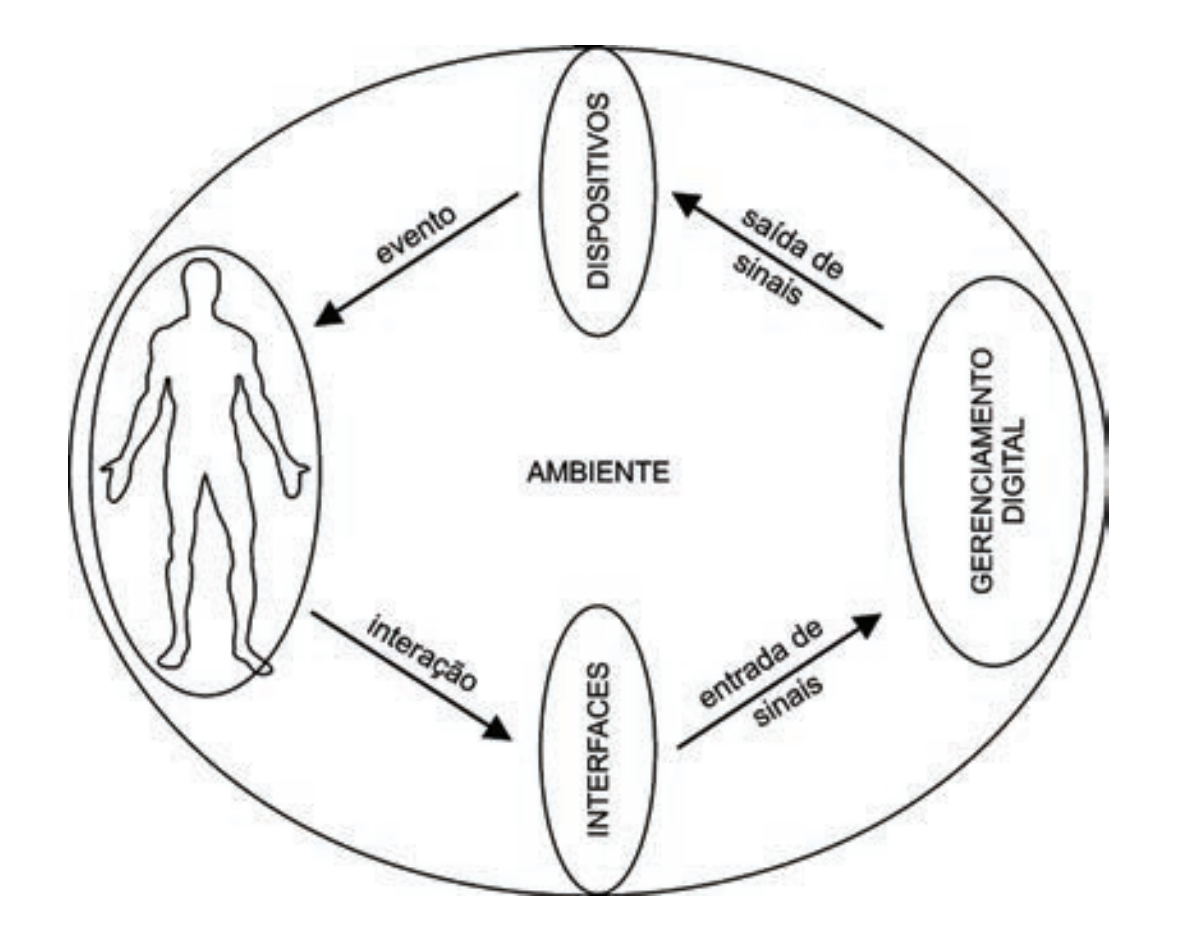
\includegraphics[width=0.8\textwidth]{./04-figuras/instalacoes_interativas}
    \label{fig:instalacoes_interativas}
\end{figure}
\vspace*{-0,9cm}
{\raggedright \fonte{\citeonline{sogabe2011}}}\\


O espaço sempre deve ser considerado para que a obra seja, de fato, uma instalação. De acordo com \citeonline[p. 6]{bochio}, no contexto das instalações interativas, o espaço se torna sensível e os movimentos mais sutis do público são capturados, provocando o diálogo com a imagem. A partir da análise realizada por \citeonline{sogabe2011} podemos afirmar que um evento é tudo que acontece dentro deste espaço. São as respostas fornecidas pelo sistema computacional que se materializam por meio dos dispositivos. Para \citeonline{domingues1998} os dispositivos compõem a cenografia, a
ambientação, mas acima de tudo acrescentam elementos internos à própria concepção
da obra. \citeonline[p. 1992]{sogabe2011} afirma que a simples presença do público no espaço, através do andar, ou de alguma ação física, pode gerar alterações no ambiente. Essas alterações são controladas por algum sistema computacional, ou como denomina o autor, através de gerenciamento digital, que recebe as informações (entrada de sinais), processa através de um programa e devolve para o ambiente no formato de informações atualizadas (saída de sinais), provocando um novo ciclo.

Para \citeonline[p. 64]{sogabe2011} a instalação interativa entende o público como essencial para o acontecimento da obra. O interator se torna um elemento físico presente na instalação e que o artista tem de considerar. Sendo assim, público e interatividade estão intimamente conectados tendo em vista que que a interação se manifesta em alguma ação proposta pelo interator. Sobre a relação do público com o espaço \citeonline[p. 6]{bochio} relata que

\begin{citacao}
Em seus deslocamentos pelo espaço, o público constrói uma trama de relações com a obra por aproximação, afastamento, retornos, paradas, transformando o que é percebido por ele. Em instalações interativas, além disso, o público tem a possibilidade de agir e interagir com a situação proposta promovendo modificações nas próprias imagens e sons:  há transformações de ordem física e não mais apenas perceptiva – o que caracteriza o termo interativo nas instalações.  \cite[p. 6]{bochio}  
\end{citacao}

Para \citeonline[p. 6]{bochio}, as instalações interativas, oferecem além de imagens ou sons, interfaces de acesso ao público, permitindo que à sua ação sejam produzidas respostas em tempo real por parte das máquinas. \citeonline{levy} define interface como sendo "todos os aparatos materiais que permitem a interação entre o universo da informação digital e o mundo ordinário" enquanto \citeonline[p. 66]{sogabe2011} afirma que "a interface é o aparato físico que capta as ações do público na instalação, a parte sensível do sistema tecnológico". \citeonline[p. 66]{sogabe2011} relata também que a interface não é apenas um aparato tecnológico, mas está diretamente relacionada à produção da poética da instalação. De acordo com \citeonline{witt}, para que qualquer tipo de interatividade aconteça, é necesária a existência de uma interface, uma tecnologia que propicie a comunicação entre o sistema e o interator. \citeonline{witt} destacam que estas interfaces devem sempre evoluir, num sentido em que se tornem cada vez mais próximas ao nosso corpo, tenham um funcionamento simples de aprender, e que, acima de tudo, sejam capazes de atender às necessidades da obra. Para \citeonline{rabello} a interface permite, através de um canal de mão dupla entre homem e máquina, que a ação do homem, por mais sutil e imperceptível que pareça, seja reconhecida, processada pela máquina e devolvida para o interator. Portanto, as interfaces se tornam um tipo de condutor, estabelecendo a interatividade e convertendo os espectadores em atores dos sistemas. \citeonline[p. 2570]{rabello2011} afirma que é por meio da interface que a troca de informação e a interação se efetiva, conectando o homem à máquina e engendrando uma atividade intensa, na qual dois mundos até então distintos são intimados a se entrecruzar. A interface provoca uma experiência interativa entre agentes, estabelecendo um novo tipo de relação entre o real e o artificial. Parafraseando \citeonline[p. 140]{arantes} podemos dizer que "é a partir da interface com o interator que a obra pode se manifestar". 

\citeonline[p. 11]{bochio} entende que, no contexto digital, a interatividade é a relação recíproca entre usuários e interfaces computacionais. A autora compreende por interfaces os dispositivos de entrada e/ou de saída que funcionam como pontes entre as ações humanas e os códigos do computador. Conclui que é, portanto, uma comunicação baseada na tradução de um código a outro, estabelecendo, assim, um código comum entre homem e máquina. 


\section{O CORPO DO OBSERVADOR NA OBRA DE ARTE INTERATIVA}
	
Numa época onde se solicita uma atuação corporal do observador dentro da obra de arte para que esta se atualize ou materialize \citeonline{sogabe} destaca que a condição do corpo do espectador adquire grande importância, pois, numa visão de um todo sistêmico, este se torna elemento constitutivo da obra. De acordo com \citeonline{vares} "quando conectado, esse corpo possuirá também alterações em sua espacialidade e fisicalidade, pois através das conexões – onde ocorre o encontro entre o orgânico e o inorgânico – seu corpo será aumentado, ampliado".

\begin{citacao}
Se a interatividade baseava-se já radicalmente nas relações tradicionais do autor, da obra e do espectador, a introdução de lógica da autonomia dessas relações torna esse relacionamento ainda mais complexo e profundo. Quer se trate de por em contato o espectador com simulações de seres humanos, organismos imaginários ou simples imagens, nota-se que os dispositivos interativos imaginados pelos artistas tendem a solicitar a participação do corpo inteiro. Existe aí uma nova forma de hibridização entre a obra e o espectador que, longe de afastar a arte para uma pretensa desmaterialização em que o corpo seria negado em proveito de puras abstrações, abre-se para outros horizontes. A tensão colocada na corporeidade retoma o lugar que perdeu, em parte, em um certo tipo de arte contemporânea. \cite[p. 37]{couchot}  
\end{citacao}

	
\citeonline{sogabe} entende que o diálogo corporal do espectador com a obra sempre existe. Segundo ele, isso ocorre mesmo nas obras de arte mais tradicionais à medida em que o próprio tamanho e a estrutura da obra provocam a aproximação, o afastamento, o andar de um lado ao outro ou o movimentar da cabeça do observador. Diz ainda que

\begin{citacao}
Nas obras mais tradicionais, até antes do modernismo, a postura do observador em geral é sempre de um corpo fixo, quase imóvel, cujos movimentos restringem-se basicamente ao olhar, que percorre a imagem, de acordo com os centros de atenção e composição dos elementos visuais existentes. \cite{sogabe} 
\end{citacao}

Segundo \citeonline{rabello} a inserção do corpo no espaço artístico foi inicialmente proposta pela arte da participação nos anos 1970 e 80. Nesta época já se articulava uma experiência sensorial por meio da ativação dos sentidos em ambientes cinéticos fosse pela utilização de óculos, pela ação de pisar, deitar ou apertar botões. Ainda de acordo \citeonline{rabello} a correlação entre o processo interativo e a experiência estética tornou-se mais evidente com o advento das tecnologias digitais à medida que estas solicitam cada vez mais a ação, a movimentação, a vivência e a conexão do homem com o ambiente virtual, promovendo situações distintas dentro de uma dimensão estética. Nesse contexto, \citeonline{sogabe} acrescenta que o corpo da obra já não existe independente do corpo do observador e que a tecnologia digital transforma os ambientes das instalações em ambientes onde o espaço projeta-se para dentro de imagens inteligentes, que se atualizam de acordo com cada participante, o qual denomina interator ou interagente.

\citeonline{vares} afirma que na interatividade o corpo dos usuários é colocado em contato direto com as tecnologias, fazendo trocas com estas através da emissão e recepção de mensagens, desenvolvendo o processo da obra. Nas palavras de \citeonline{witt}, "a interatividade também proporciona uma fricção: a do corpo do usuário, orgânico, com um sistema tecnológico, artificial". Para \citeonline{vares}, neste contexto, a realização da obra não pode ser atribuída apenas ao artista, pois o público irá decidir se empresta ou não o seu corpo ao trabalho. Ela acrescenta que existe uma mudança de paradigma da própria experiência corporal tendo em vista que esses experimentos acontecem publicamente, onde qualquer ação executada pelo interator pode ser vista por outras pessoas presentes no espaço, que podem vir a julgá-lo. Esse fato, pode interferir no próprio desenrolar da obra, fazendo com que o usuário se dedique mais ou menos a participar efetivamente da mesma. \citeonline{witt} concluem que "durante o processo das obras, ambos são convidados a trabalhar em conjunto para que a proposta artística tenha sucesso. Afinal, é ao corpo que pertencem nossas sensações e percepções, que são justamente os campos afetados por instalações interativas".
